%卒論概要テンプレート ver. 4.0

\documentclass[uplatex,twocolumn,dvipdfmx]{jsarticle}
\usepackage[top=22mm,bottom=22mm,left=22mm,right=22mm]{geometry}
\setlength{\columnsep}{11mm}
\usepackage[T1]{fontenc}
\usepackage{txfonts}
\usepackage[expert,deluxe]{otf}
\usepackage[dvipdfmx,hiresbb]{graphicx}
\usepackage[dvipdfmx]{hyperref}
\usepackage{pxjahyper}
\usepackage{secdot}





%タイトルと学生番号,名前だけ編集すること
\title{\vspace{-5mm}\fontsize{14pt}{0pt}\selectfont Word2vecを用いたパラグラフ・ライティング}
\author{\normalsize プロジェクトマネジメントコース 矢吹研究室 1442069 氏名 須山 武弘}
\date{}
\pagestyle{empty}
\begin{document}
\fontsize{10.5pt}{\baselineskip}\selectfont
\maketitle





%以下が本文
\section{序論}\label{序論}

レポートや論文を書く際には,読みやすく,論理的な文章を書くことが大切である.読みやすく,論理的な文章とは,伝えたいことが読み手に伝わり,段落内の話題が統一されている事が必要である.論理的文章は学習をしなければ書けるようにはならない.欧米では,半年~1年をかけて勉強することがある.

パラグラフ・ライティング(Paragraph writing)とは,論理的文章を書くための世界標準の書き方である\cite{02}.冒頭にトピックとなる文を配置し,後ろに補助する文を配置するピラミッド構造的な文章の書き方である.最初にトピックとなる文を配置することにより,結論がはっきりし,内容の理解が深まることや,冒頭にトピックを記すことで,速読が可能になるなど,多数のメリットがある.

本研究では,Word2vecを利用し,単語の意味をベクトル化し,定量的結果から,パラグラフ・ライティングの補助ができるのではないかと考えられる\cite{01}.

\section{目的}
本研究では,文字列である文章をベクトルで表し,パラグラフ・ライティングの補助をすることが目的である.段落内文章の意味のベクトルをWord2vecで定量的に表す.結果として,同じようなベクトルの位置に分布すると,定量的に意味が同じであると考えられる.

\section{手法}

本研究では,Word2vecを用いて文章をベクトル化し,数値的面から論理的文章作成を補助する.通常,文章は定量的に表すことができないが,Word2vecは,単語をベクトルとして数値へ変換できるニューラルネットのことである.文章をベクトルへ変換することによって単語の意味を個人の主観ではなく,定量的に表すことができる.

対象文章の形態素解析をMecabで実行し,Wikipediaの情報を利用したコーパスである,東北大学乾・岡崎研究室「日本語 Wikipedia エンティティベクトル」を利用し,単語のベクトル化を行い,主成分分析の結果を図示する.


\section{結果}
手法にあるように,Word2vecを用いて文章のベクトル化を行った出力結果が図1である.過去に人間による添削済みの文章であり,同じ色のベクトルが同段落の文章のベクトルである.
\begin{figure}[h]
\centering
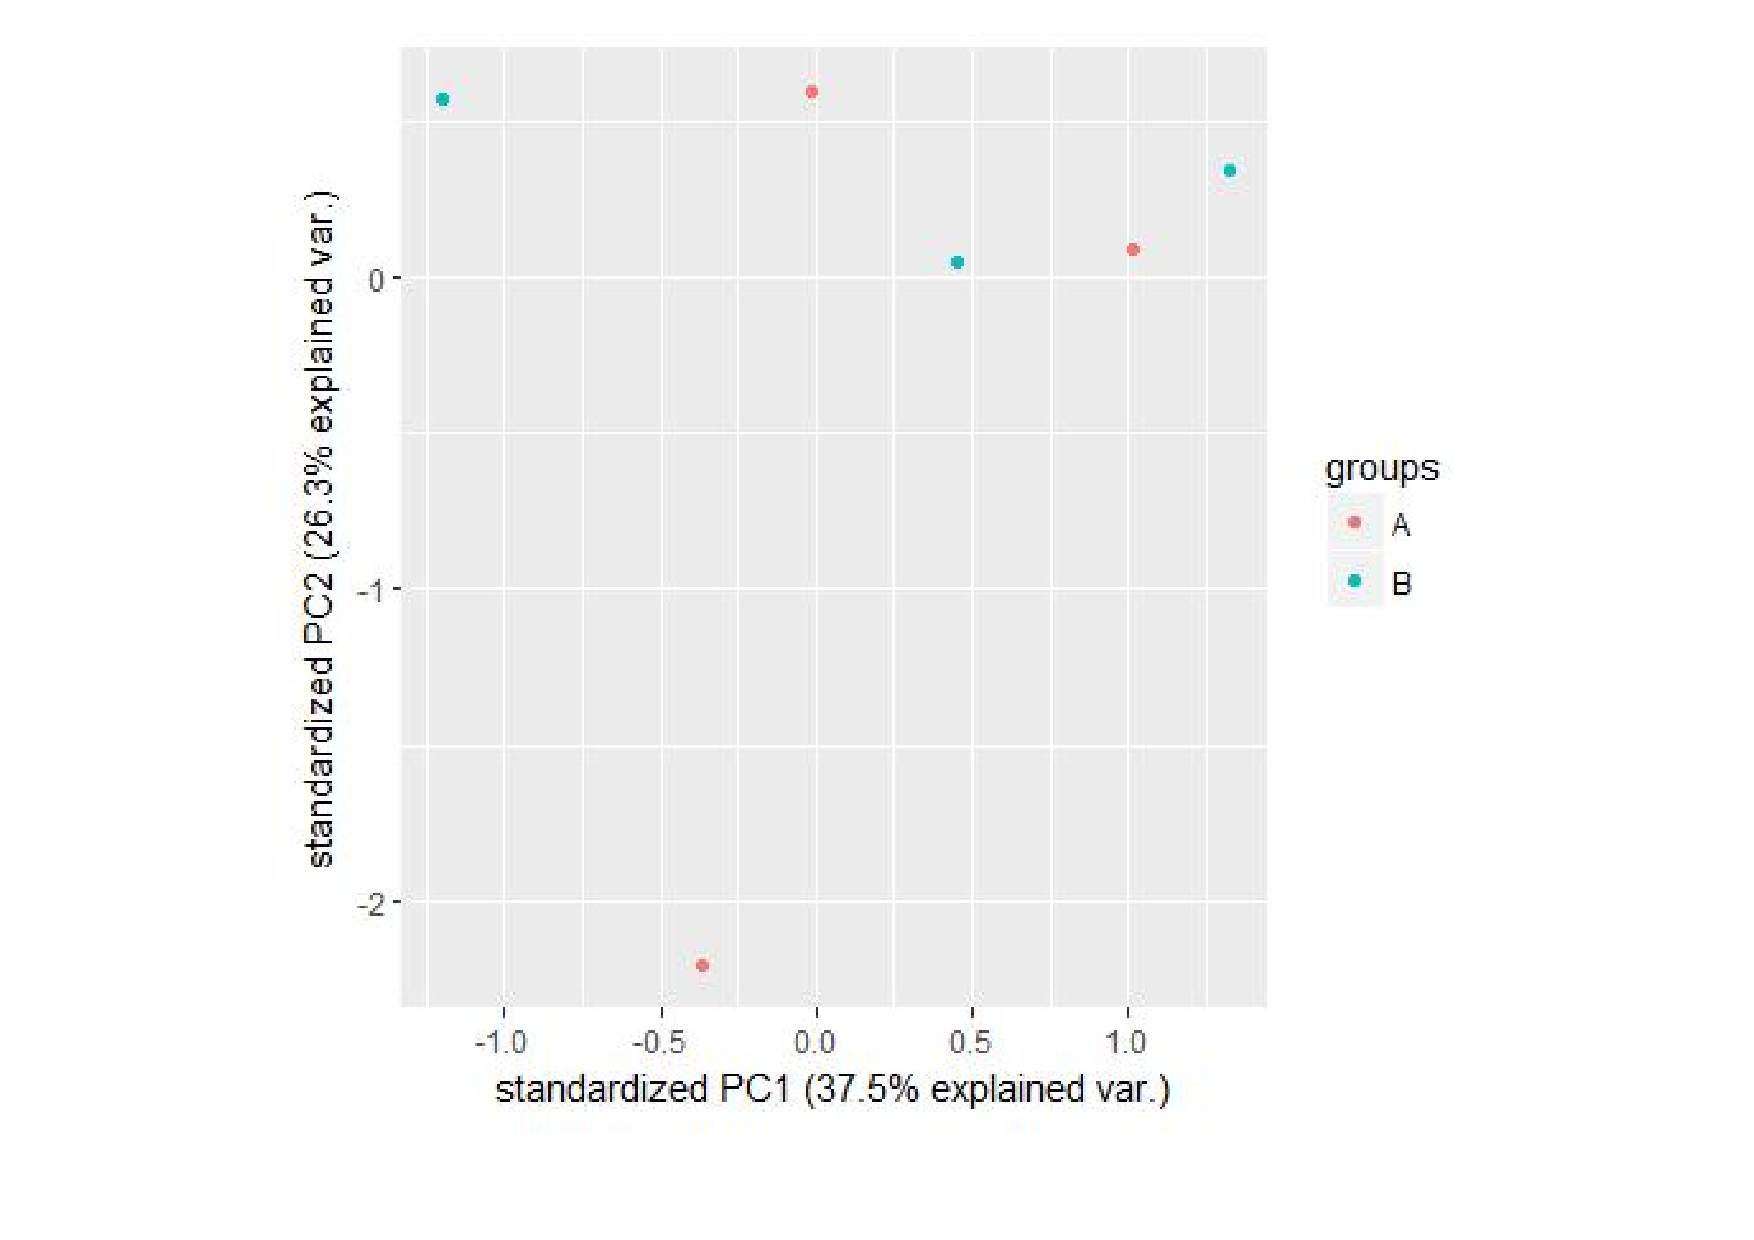
\includegraphics[width=5cm]{02.pdf}
\caption{word2vecによる分析結果}\label{分析結果}
\end{figure}


\section{考察}

同段落にもかかわらず,ベクトルは散らばって分布している事がわかる.この内容では,それぞれの文章が違う話題を示していると考えられる.

パラグラフ・ライティングにおける考え方として,段落内の文は冒頭の一文を補助する文であることから,本研究の結果から,うまくパラグラフ・ライティングができていないという結果になったと考えられる.

\section{結論}

今回の結果から,Word2vecを用いて数値によって文章を見ていくことで,個人の主観だけでなく,定量的に文章の書き方を定義できることも期待される.

\bibliographystyle{junsrt}
\bibliography{biblio}%「biblio.bib」というファイルが必要.

\end{document}
